% Created 2017-02-22 Wed 18:10
% Intended LaTeX compiler: pdflatex
\documentclass[11pt]{article}
\usepackage[utf8]{inputenc}
\usepackage[T1]{fontenc}
\usepackage{graphicx}
\usepackage{grffile}
\usepackage{longtable}
\usepackage{wrapfig}
\usepackage{rotating}
\usepackage[normalem]{ulem}
\usepackage{amsmath}
\usepackage{textcomp}
\usepackage{amssymb}
\usepackage{capt-of}
\usepackage{hyperref}
\date{\today}
\title{}
\hypersetup{
 pdfauthor={},
 pdftitle={},
 pdfkeywords={},
 pdfsubject={},
 pdfcreator={Emacs 25.1.1 (Org mode 9.0.3)}, 
 pdflang={English}}
\begin{document}

\section{Pr. 30}
\label{sec:org2eeb131}
\subsection{a) Gradient Method}
\label{sec:org73dce56}
The following is a graph of the convergence rate for the gradient method. Here  \(A\) is a randomly generated 50x50 matrix that satisfied the given constraints. \(\alpha = 0.02\), \(\beta = 0.32\) and a calculated \(P* = -.0013\). 


\begin{center}
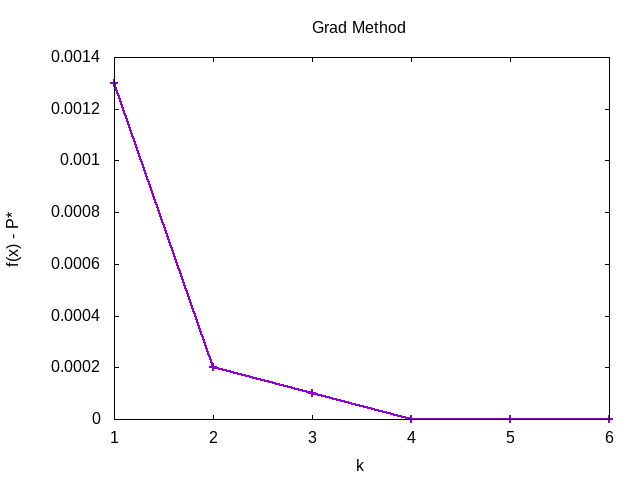
\includegraphics[width=.9\linewidth]{grad.png}
\end{center}

\subsection{b) Newton Method}
\label{sec:org05ed1f5}
I used the same parameters as above for Newton method, and the algorithm converged to \(P*\) in two iterations rather than 6.
\end{document}